% Matboard Bridge - small-scale box girder bridge
% Copyright © 2023 Nabeth Ghazi
%
% This program is free software: you can redistribute it and/or modify
% it under the terms of the GNU General Public License as published by
% the Free Software Foundation, version 3.
%
% This program is distributed in the hope that it will be useful,
% but WITHOUT ANY WARRANTY; without even the implied warranty of
% MERCHANTABILITY or FITNESS FOR A PARTICULAR PURPOSE.  See the
% GNU General Public License for more details.
%
% You should have received a copy of the GNU General Public License
% along with this program. If not, see <http://www.gnu.org/licenses/>.

\documentclass[11pt, fleqn]{article}
\usepackage[utf8]{inputenc}
\usepackage[letterpaper, margin=1in]{geometry}
\usepackage{setspace}
\setstretch{1.25}
\usepackage[labelsep=period, labelfont=bf]{caption}

\usepackage{hyperref}
\hypersetup{colorlinks= true,urlcolor= black,linkcolor= black}

\usepackage{xcolor}
\newcommand{\mathhl}[1]{\colorbox{yellow}{$\displaystyle #1$}}

\usepackage{siunitx}
\sisetup{reset-math-version=false}

\usepackage{listings}
\lstset{language=MATLAB,frame=single,basicstyle=\ttfamily\small,showstringspaces=false,columns=flexible,literate={\ }{{\ }}1}

\usepackage{mathtools}
\usepackage{amsmath}

\begin{document}

\clearpage
\pagenumbering{roman}
\title{Matboard Bridge\\ \textbf{Design Calculations}}
\author{Nabeth Ghazi}
\date{}
\maketitle

\tableofcontents

\clearpage
\pagenumbering{arabic}

\section{Design 0}

\subsection{Hand Calculations}

\setcounter{subsubsection}{-1}
\subsubsection{Cross Section}
\begin{align*}
    \bar{y} & = \frac{\sum{A_iy_i}}{\sum A_i} = \frac{\sum{b_ih_iy_i}}{\sum{b_ih_i}}                                                                    \\
            & = \frac{(80)(1.27)(0.635)+(100)(1.27)(75.63)+2(1.27)(73.73)(38.135)+2(5)(1.27)(74.365)}{(80)(1.27)+(100)(1.27)+2(1.27)(73.73)+2(5)(1.27)} \\
            & = \SI{41.4296}{\mm} = \mathhl{\SI{41.4}{\mm}}
\end{align*}
\begin{align*}
    I = \sum{I_i+A_i{d_i}^2} & = \frac{b_i{h_i}^3}{12}+b_ih_i\left(\bar{y}-y_i\right)^2                      \\
                             & = \frac{(80)(1.27)^3}{12}+(80)(1.27)[(41.4296)-(0.635)]^2                     \\
                             & +\frac{(100){(1.27)}^3}{12}+(100)(1.27)[(41.4296)-(75.63)]^2                  \\
                             & +2\left(\frac{(1.27)(73.73)^3}{12}+(1.27)(73.73)[(41.4296)-(38.135)]^2\right) \\
                             & +2\left(\frac{(5)(1.27)^3}{12}+(5)(1.27)[(41.4296)-(74.365)]^2\right)         \\
                             & = \SI{418.309e3}{\mm^4} = \mathhl{\SI{418e3}{\mm^4}}
\end{align*}

\subsubsection{Flexural Tension Failure}
\[ M_{\mathrm{max}} = \SI{69445.3}{\N\mm} \quad \text{at} \quad x_{\mathrm{train}} \in \{\SI{557}{\mm},\SI{644}{\mm}\} \]
\[ y_{bot} = \bar{y}-0 = \SI{41.4296}{\mm} \]
\[ \sigma_{\mathrm{demand}} = \frac{M_{max}y_{bot}}{I} = \frac{(69445.3)(41.4296)}{(\SI{418.309e3}{})} = \SI{6.87791}{\MPa} \]
\[ \sigma_{\mathrm{tension}} = \SI{30}{\MPa} \]
\[ {\mathrm{FOS}}_{\mathrm{tension}} = \frac{\sigma_{\mathrm{tension}}}{\sigma_{\mathrm{demand}}} = \frac{(30)}{(6.87791)} = 4.3618 = \mathhl{4.36} \]

\subsubsection{Flexural Compression Failure}
\[ M_{\mathrm{max}} = \SI{69445.3}{\N\mm} \quad \text{at} \quad x_{\mathrm{train}} \in \{\SI{557}{\mm},\SI{644}{\mm}\} \]
\[ y_{top} = \bar{y}-h = (41.4296)-(76.27) = \SI{-34.8404}{\mm} \]
\[ \sigma_{\mathrm{demand}} = \frac{M_{max}y_{top}}{I} = \frac{(69445.3)(-34.8404)}{(\SI{418.309e3}{})} = \SI{-5.78401}{MPa} \]
\[ \sigma_{\mathrm{comp}} = \SI{-6}{\MPa} \]
\[ {\mathrm{FOS}}_{\mathrm{comp}} = \frac{\sigma_{\mathrm{comp}}}{\sigma_{\mathrm{demand}}} = \frac{(-6)}{(-5.78401)} = 1.03734 = \mathhl{1.037} \]

\subsubsection{Material Shear Stress Failure}
\[ V_{\mathrm{max}} = \SI{240}{\N} \quad \text{at} \quad x_{\mathrm{train}} = \SI{1}{\mm} \]
\begin{align*}
    Q(\bar{y}) & = \sum{A_id_i}                                                                                           \\
               & = 2(1.27)(41.4296-1.27)\left(\frac{41.4296-1.27}{2}\right)+(80)(1.27)\left(41.4296-\frac{1.27}{2}\right) \\
               & = \SI{6192.98}{\MPa}
\end{align*}
\[ b(\bar{y}) = 2(1.27) = \SI{2.54}{\mm} \]
\[ \tau_{demand} = \frac{VQ}{Ib} = \frac{(240)(6192.98)}{(\SI{418.309e3}{})(2.54)} = \SI{1.39888}{\MPa} \]
\[ \tau_{max} = \SI{4}{\MPa} \]
\[ {\mathrm{FOS}}_{\mathrm{shear}} = \frac{\tau_{max}}{\tau_{demand}} = \frac{(4)}{(1.39888)} = 2.85943 = \mathhl{2.86} \]

\subsubsection{Glue Shear Stress Failure}
\[ V_{\mathrm{max}} = \SI{240}{\N} \quad \text{at} \quad x_{\mathrm{train}} = \SI{1}{\mm} \]
\[ Q(75) = \sum{A_id_i} = (100)(1.27)\left(34.8404-\frac{1.27}{2}\right) = \SI{4344.09}{\MPa} \]
\[ b(75) = 2(5+1.27) = \SI{12.54}{\mm} \]
\[ \tau_{demand} = \frac{VQ}{Ib} = \frac{(240)(4344.09)}{(\SI{418.309e3}{})(12.54)} = \SI{198.754e-3}{\MPa} \]
\[ \tau_{glue} = \SI{2}{\MPa}\]
\[ {\mathrm{FOS}}_{\mathrm{glue}} = \frac{\tau_{max}}{\tau_{demand}} = \frac{(2)}{(\SI{198.754e-3}{})} = 10.0627 = \mathhl{10.06} \]

\subsubsection{Case 1 Flexural Buckling Failure}
\[ M_{\mathrm{max}} = \SI{69445.3}{\N\mm} \quad \text{at} \quad x_{\mathrm{train}} \in \{\SI{557}{\mm},\SI{644}{\mm}\} \]
\[ \sigma_{\mathrm{demand}} = \frac{M_{\mathrm{max}}y_{\mathrm{top}}}{I} = \frac{(69445.3)(34.8404)}{(\SI{418.309e3}{})} = \SI{5.78401}{\MPa} \]
\[ b_{\mathrm{crit,1}} = 80-1.27 = \SI{78.73}{\mm} \]
\[ \sigma_{\mathrm{crit,1}} = \frac{K\pi^2E}{12\left(1-\mu^2\right)}\left(\frac{t}{b_{\mathrm{crit,1}}}\right)^2 = \frac{\left(4\right)\pi^2\left(4000\right)}{12\left[1-\left(0.2\right)^2\right]}\left(\frac{1.27}{78.73}\right)^2 = \SI{3.56693}{\MPa} \]
\[ {\mathrm{FOS}}_{\mathrm{buck,1}} = \frac{\sigma_{\mathrm{crit,1}}}{\sigma_{\mathrm{demand}}} = \frac{(3.56693)}{(5.78401)} = 0.616688 = \mathhl{\SI{617e-3}{}} \]

\subsubsection{Case 2 Flexural Buckling Failure}
\[ M_{\mathrm{max}} = \SI{69445.3}{\N\mm} \quad \text{at} \quad x_{\mathrm{train}} \in \{\SI{557}{\mm},\SI{644}{\mm}\} \]
\[ \sigma_{\mathrm{demand}} = \frac{M_{\mathrm{max}}y_{\mathrm{top}}}{I} = \frac{(69445.3)(34.8404)}{(\SI{418.309e3}{})} = \SI{5.78401}{\MPa} \]
\[ b_{\mathrm{crit,2}} = \frac{100-80}{2}+\frac{1.27}{2} = \SI{10.635}{\mm} \]
\[ \sigma_{\mathrm{crit,2}} = \frac{K\pi^2E}{12\left(1-\mu^2\right)}\left(\frac{t}{b_{\mathrm{crit,2}}}\right)^2 = \frac{\left(0.425\right)\pi^2\left(4000\right)}{12\left[1-\left(0.2\right)^2\right]}\left(\frac{1.27}{10.635}\right)^2 = \SI{20.7696}{\MPa} \]
\[ {\mathrm{FOS}}_{\mathrm{buck,2}} = \frac{\sigma_{\mathrm{crit,2}}}{\sigma_{\mathrm{demand}}} = \frac{(20.7696)}{(5.78401)} = 3.59087 = \mathhl{3.59} \]

\subsubsection{Case 3 Flexural Buckling Failure}
\[ M_{\mathrm{max}} = \SI{69445.3}{\N\mm} \quad \text{at} \quad x_{\mathrm{train}} \in \{\SI{557}{\mm},\SI{644}{\mm}\} \]
\[ y_{\mathrm{crit,3}} = y_{top}-1.27 = 34.8404-2.54 = \SI{33.5704}{\mm} \]
\[ \sigma_{\mathrm{demand}} = \frac{M_{\mathrm{max}}y_{\mathrm{crit,3}}}{I} = \frac{(69445.3)(33.5704)}{(\SI{418.309e3}{})} = \SI{5.57317}{\MPa} \]
\[ b_{\mathrm{crit,3}} = y_{top}-\frac{3(1.27)}{2} = 34.8404-1.905 = \SI{32.9354}{mm} \]
\[ \sigma_{\mathrm{crit,3}} = \frac{K\pi^2E}{12\left(1-\mu^2\right)}\left(\frac{t}{b_{\mathrm{crit,3}}}\right)^2 = \frac{\left(6\right)\pi^2\left(4000\right)}{12\left[1-\left(0.2\right)^2\right]}\left(\frac{1.27}{32.9354}\right)^2 = \SI{30.5731}{\MPa} \]
\[ {\mathrm{FOS}}_{\mathrm{buck,3}} = \frac{\sigma_{\mathrm{crit,3}}}{\sigma_{\mathrm{demand}}} = \frac{(30.5731)}{(5.57317)} = 5.48576 = \mathhl{5.49} \]

\subsubsection{Shear Buckling Failure}
\[ \tau_{demand} = \frac{VQ(\bar{y})}{Ib(\bar{y})} = \frac{(240)(6192.98)}{(\SI{418.309e3}{})(2.54)} = \SI{1.39888}{\MPa} \]
\[ b_{\mathrm{crit,4}} = 75-1.25 = \SI{73.73}{\mm} \]
\[ a_{\mathrm{crit,4}} = 1200/3 = \SI{400}{\mm} \]
\[ \tau_{\mathrm{crit}} = \frac{K\pi^2E}{12\left(1-\mu^2\right)}\left[\left(\frac{t}{b_{\mathrm{crit,4}}}\right)^2+\left(\frac{t}{a_{\mathrm{crit,4}}}\right)^2\right] = \frac{\left(5\right)\pi^2\left(4000\right)}{12\left[1-\left(0.2\right)^2\right]}\left[\left(\frac{1.27}{73.73}\right)^2+\left(\frac{1.27}{400}\right)^2\right] = \SI{5.25662}{\MPa} \]
\[ {\mathrm{FOS}}_{\mathrm{buck,4}} = \frac{\tau_{\mathrm{crit}}}{\tau_{\mathrm{demand}}} = \frac{(5.25662)}{(1.39888)} = 3.75773 = \mathhl{3.76} \]

\subsubsection{$\mathrm{FOS}$ and $P_{\mathrm{fail}}$}
\begin{align*}
    \mathrm{FOS} & = \mathrm{min}\left\{{\mathrm{FOS}}_{\mathrm{tension}},{\mathrm{FOS}}_{\mathrm{comp}},{\mathrm{FOS}}_{\mathrm{shear}},{\mathrm{FOS}}_{\mathrm{glue}},{\mathrm{FOS}}_{\mathrm{buck,1}},{\mathrm{FOS}}_{\mathrm{buck,2}},{\mathrm{FOS}}_{\mathrm{buck,3}},{\mathrm{FOS}}_{\mathrm{buck,4}}\right\} \\
                 & = {\mathrm{FOS}}_{\mathrm{buck,1}}                                                                                                                                                                                                                                                               \\
                 & = 0.616688 = \mathhl{\SI{617e-3}{}}
\end{align*}
\[ P_{\mathrm{fail}} = \mathrm{FOS}\times{P}_{demand} = (0.616688)(400) = \SI{246.675}{\N} = \mathhl{\SI{247}{\N}} \]

\subsection{Intermediate Code Calculations}
\begin{lstlisting}[]
ybar = 41.431094351923186
I = 4.183522089994237e+05
max(M) = 6.944533333333337e+04
ybot = 41.431094351923186
S_tens_app = 6.877449421183897
ytop = -34.838905648076810
S_comp_app = -5.783163955284811
Q_max = 6.193283330576414e+03
b_centroid = 2.540000000000000
T_max_app = 1.398802523651935
max(V) = 2.400000000000000e+02
Q_glue = 4.343896017305791e+03
b_glue = 12.539999999999999
T_glue_app = 0.198724338232346
S_buck1_app = 5.783163017719362
S_buck1_ult = 3.566926726812471
S_buck2_app = 5.783163017719362
S_buck2_ult = 20.769624320288855
S_buck3_app = 5.572346458284259
S_buck3_ult = 30.573884061715709
T_buck_app = 1.398802523651935
T_buck_ult = 5.256619850378164    
\end{lstlisting}

All intermediate hand calculations perfectly match their respective computer-generated values to slide rule precision, excluding \lstinline{T_glue_app} which is has a deviation of
\[ \varepsilon = \left|0.198724338232346-\SI{198.754e-3}{}\right| < \SI{30.0e-6}{} \]
which is considered consistent with zero.

\subsection{Code Output}

\subsubsection{$\mathrm{FOS}$ and $P_{\mathrm{fail}}$}
\begin{lstlisting}[]
FOS_tens = 4.36
FOS_comp = 1.037
FOS_shear = 2.86
FOS_glue = 10.06
FOS_buck1 = 0.617
FOS_buck2 = 3.59
FOS_buck3 = 5.49
FOS_buckV = 3.76
    
minFOS = 0.617
P_fail = 247 N
\end{lstlisting}

All hand calculated FOS and failure load values perfectly match their respective computer-generated values to slide rule precision.

\subsubsection{Shear Force and Bending Moment Capacities Diagram}
\begin{figure}[h]
    \centering
    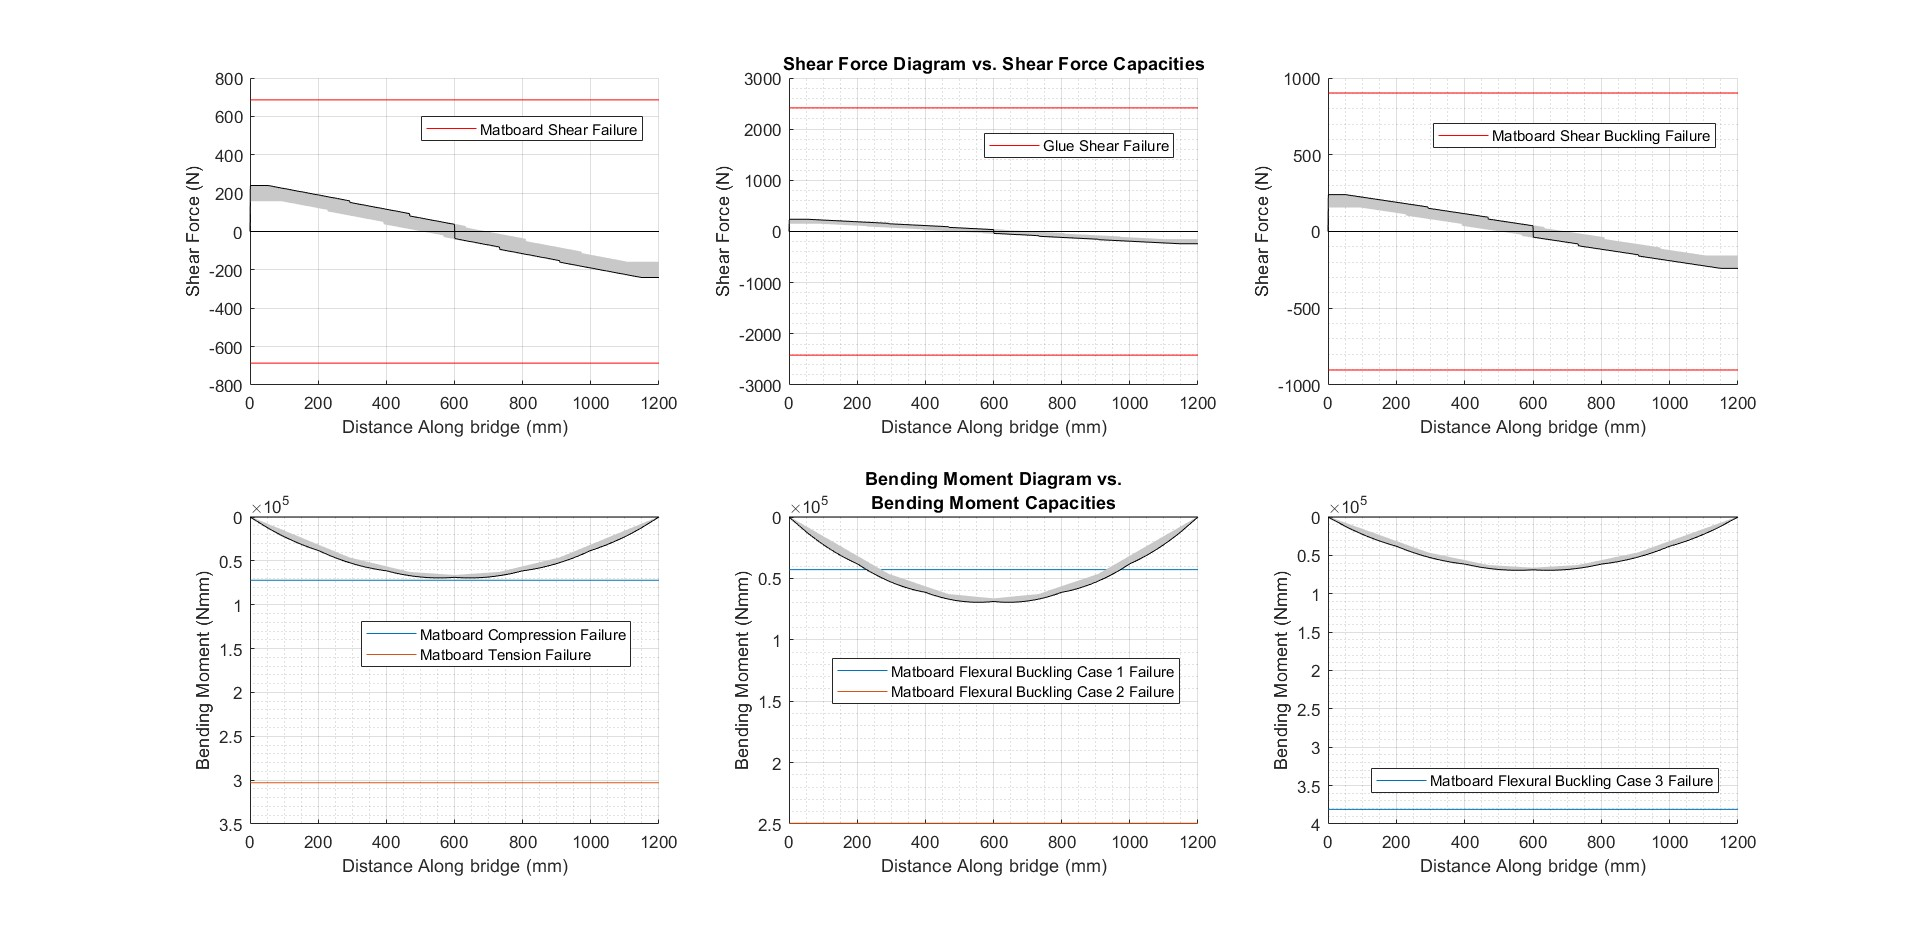
\includegraphics[width=\linewidth]{../../img/design-0.jpg}
    \caption{Subplot depicting the shear force and bending moment capacities of design 0 vs. shear force and bending moment envelope as a function of distance along the bridge.}
\end{figure}

\section{Final Design}

\subsection{Code Output}

\subsubsection{$\mathrm{FOS}$ and $P_{\mathrm{fail}}$}
\begin{lstlisting}[]
FOS_tens = 6.65
FOS_comp = 3.13
FOS_shear = 3.62
FOS_glue = 3.45
FOS_buck1 = 19.13
FOS_buck2 = 45.2
FOS_buck3 = 30.9
FOS_buckV = 3.05
    
minFOS = 3.05
P_fail = 1220 N    
\end{lstlisting}

\subsubsection{Shear Force and Bending Moment Capacities Diagram}
\begin{figure}[h]
    \centering
    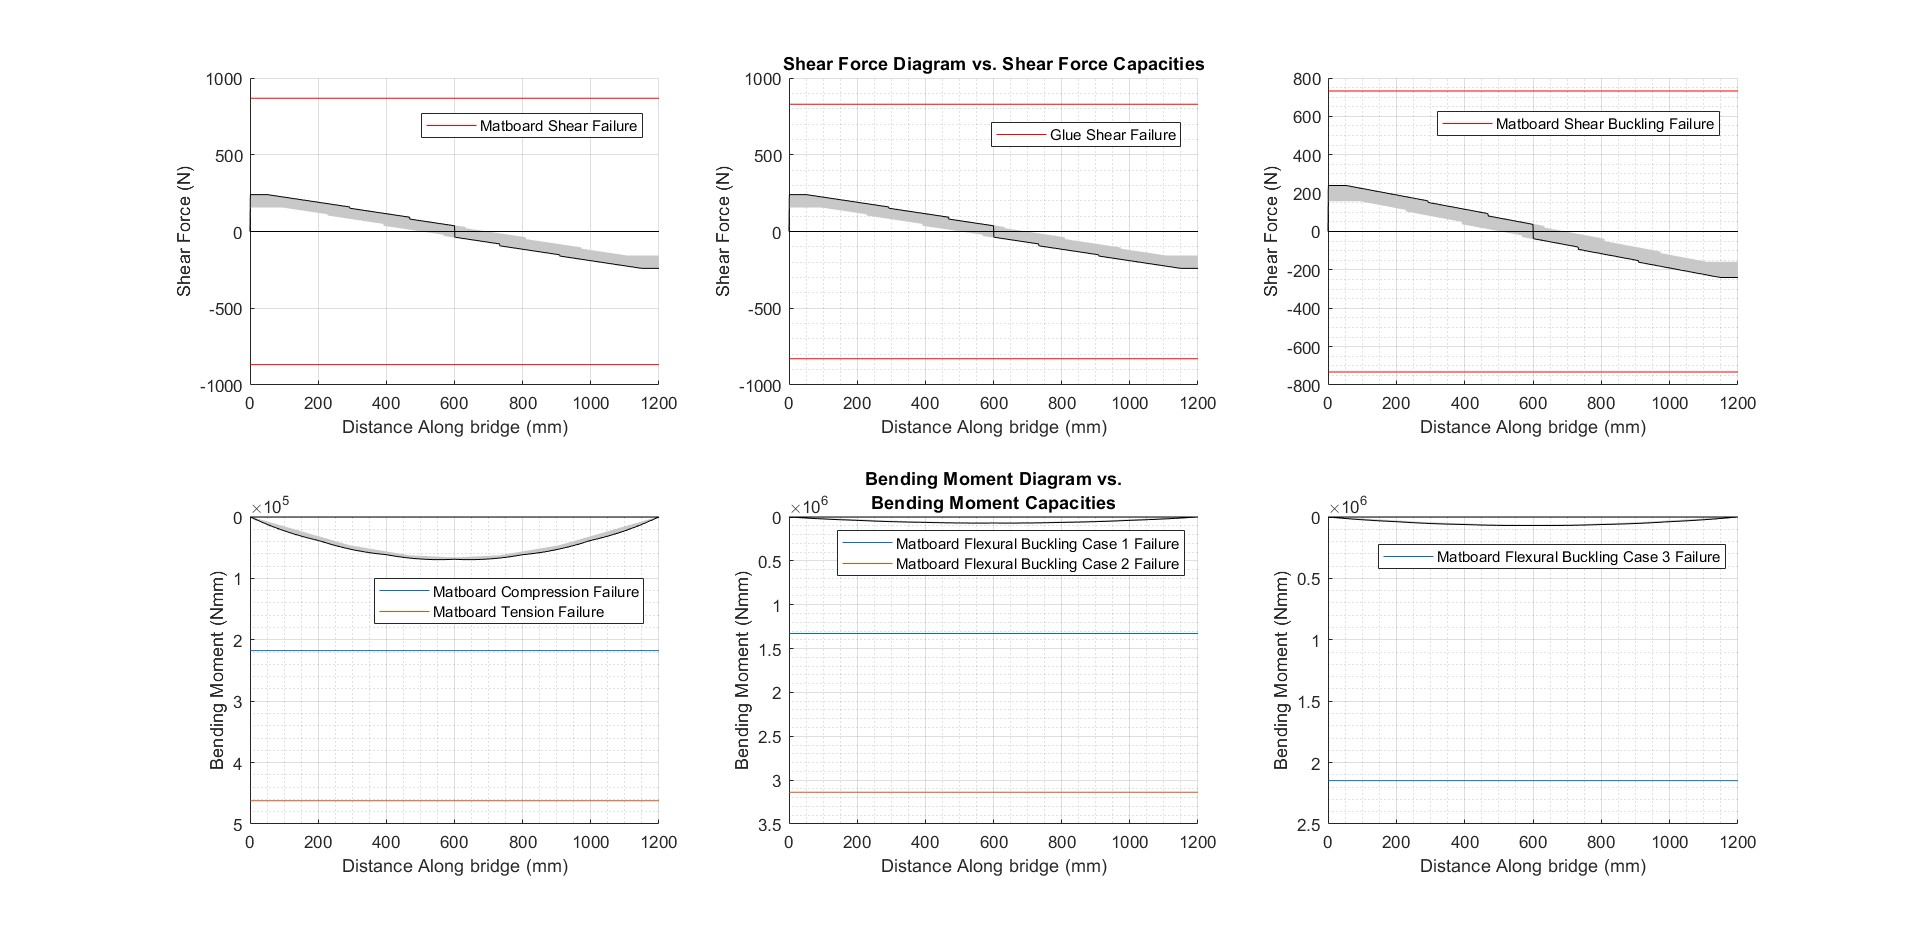
\includegraphics[width=\linewidth]{../../img/final-design.jpg}
    \caption{Subplot depicting the shear force and bending moment capacities of the final design vs. shear force and bending moment envelope as a function of distance along the bridge.}
\end{figure}

\end{document}